\section{Other Insights}

\subsection{Try to predict the medal of the 2032 Olympics}

\begin{figure}[h]
\centering
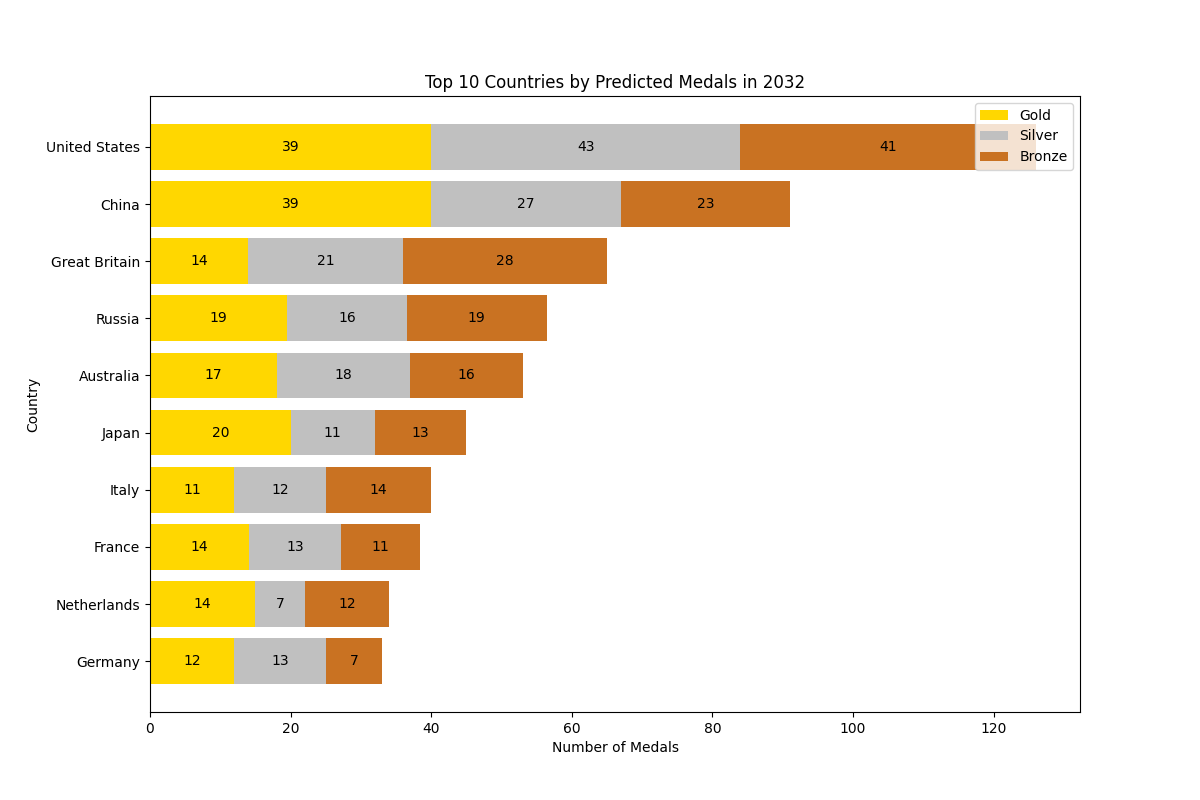
\includegraphics[width=1.1\textwidth]{../figures/2032.png}
\caption{Predicted Medal Counts for the 2032 Olympics}
\label{fig:medal_prediction}
\end{figure}

The prediction of 2032 Olympics is rather difficult because of the uncertainty of the future and almost no information of the 2032 Olympics. In \textbf{Figure \ref{fig:medal_prediction}}, we've tried to make some prediction with our comprehensive PRE model, taking all effects into account.Although the prediction may not be accurate enough, it can still serve as a reference.

\subsection{Greatness and the strategy of the country Olympic committees}


\section{Strength and Weakness}

\subsection{Strength}

\begin{itemize}
\item We analyze the problem based on thermodynamic formulas and laws, so that the model we established is of great validity.

\item Our model is fairly robust due to our careful corrections in consideration of real-life situations and detailed sensitivity analysis.

\item Via Fluent software, we simulate the time field of different areas throughout the bathtub. The outcome is vivid for us to understand the changing process.

\item We come up with various criteria to compare different situations, like water consumption and the time of adding hot water. Hence an overall comparison can be made according to these criteria.

\item Besides common factors, we still consider other factors, such as evaporation and radiation heat transfer. The evaporation turns out to be the main reason of heat loss, which corresponds with other scientist’s experimental outcome.
\end{itemize}

\subsection{Weakness}

\begin{itemize}
\item Having knowing the range of some parameters from others’ essays, we choose a value from them to apply in our model. Those values may not be reasonable in reality.

\item Although we investigate a lot in the influence of personal motions, they are so complicated that need to be studied further.

\item Limited to time, we do not conduct sensitivity analysis for the influence of personal surface area.
\end{itemize}

\subsection{Further Discussions}